\section{Evaluation}\label{evaluation}
% \begin{figure}[t]
% \centering
% \includegraphics[width=1.0\linewidth, trim=0cm 0cm 0cm 0cm]{boxplot.pdf}
% \caption{Distribution of cumulative contact duration for each node pair}
% \label{box}
% \end{figure}
This section presents evaluation results that show the effectiveness of x-ego betweenness and the efficiency of our algorithm for computing x-ego betweenness.
Section~\ref{data_construction} describes the wireless trace data sets and the methods for constructing x-ego networks in our evaluations.
Our evaluation results demonstrate that x-ego betweenness is a more accurate approximation of betweenness than ego betweenness (Section~\ref{accuracy}) and our algorithm more quickly computes x-ego betweenness than the Brandes algorithm (Section~\ref{efficiency}).


% In this section, we present the proposed measure and algorithm's evaluation results obtained on the diverse mobility trace data sets. On the data sets, we compute the x-ego betweenness and ego betweenness of a DTN node $v$ (i.e., $\BX{v}$ and $\BE{v}$) and compare them with the globally computed betweenness (i.e., $\B{v}$). We also focus to study the execution time of the proposed algorithm to get the x-ego betweenness.

%During performing the evaluation, we have focused to uncover the followings: 1) the correlation between $\BX{v}$ and $\B{v}$ is higher than the one between $\BE{v}$ and $\B{v}$, and 2) the proposed algorithm to get the x-ego betweenness is more efficient than the Brandes algorithm. 

% In this evaluation, we are not trying to compare the actual betweenness values of each node but rather to determine which nodes are more central than others.

% In this analysis, we are not trying to determine the actual betweenness value of each node but to
% determine which nodes are more central than others. So, we use the Spearman's rank correlation coefficient which measures the strength of association between two ranked variables. All betweenness values for each DTN node are ranked separately by putting the values in order and numbering them: the lowest value is given rank 1, the next lowest is given rank 2 and so on. Then, we conduct the Spearman rank correlation on the new ranked variables. The correlation value can vary between -1.0 and +1.0. The closer value is to +1.0, the stronger the association between the values.     
 
\subsection{Data Sets and X-Ego Network Construction}\label{data_construction}
   
% \begin{figure}[th]
% \centering
% \includegraphics[width=1.0\linewidth, trim=0cm 0cm 0cm 0cm]{density.pdf}
% \caption{box plot}
% \label{box}  
% \end{figure} 

% For simulations, we use the real mobility trace data sets \cite{cambridge-haggle-2009-05-29} referred to as {\em Infocom05}, {\em Infocom06},  {\it Cambridge} and {\it Intel}. 
Our evaluations used the CRAWDAD trace data sets \cite{cambridge-haggle-2009-05-29} that are referred to as {\em Infocom05}, {\em Infocom06},  {\it Cambridge} and {\it Intel}.
%Each characteristic of the data sets is summarized in Table \ref{data_set}. 
Table \ref{data_set} provides details of these data sets. 
Each of these data sets includes a number of traces of Bluetooth sightings by groups of users carrying small devices (iMotes) for a number of days. 
%They covers the diverse network scales (from small to large number of nodes) and the diversity of connection densities (from sparse to dense contacts). 
These data sets cover a variety of network scales (from small to large number of nodes) and contact densities (from sparse to dense contacts). 
For each data set, Table \ref{data_set} shows the mean and median values of accumulated contact duration per node pair. 
The disparity between these values indicates that most node pairs make contacts for a short amount of time and there are a few outliers representing long contact durations.
%The detailed characteristics of these data sets can be found in previous works listed by~\cite{crawdad-papers}. 
Further details of the data sets can be found from the CRAWDAD website~\cite{crawdad-papers}. 
% In our simulation, a social link between two DTN nodes is created if the accumulated contact duration between two nodes is above a given threshold denoted by $\theta$. 
In our evaluations, a social link between two nodes was assumed if the accumulated contact duration between the two nodes was above a given threshold $\theta$. 
% For each data set, we determined nine threshold duration values, which are symbolized by the density ratio $10\%, 20\%, \cdots, 90\%$.
For each data set, we determined nine duration threshold values that correspond to the link addition ratio of $10\%, 20\%, \cdots, 90\%$.  
%More specifically, we first assume that the density ratio $100\%$ indicates $\theta=0$ sec., which means at least one (very short) contact between two nodes corresponds to the creation of an edge between them and they get the relationship of social neighbor each other. 
More specifically, for the link addition ratio of $100\%$, we set the contact duration threshold ($\theta$) to 0 seconds.
In this case, any contact between two nodes led to the addition of a social link between the nodes.
Then, we determined each duration threshold value (e.g., $\theta=141, 468, \cdots, 5921$ in the case of {\em Infocom05}) so that $90\%$, $80\%$, $\cdots$, $10\%$ of all possible social links would be added (Table \ref{data_set}). 
% It is noted that the duration threshold values corresponding to the density ratio $50\%$ for each data set are equal to the median values of the accumulated contact duration.
It should be noted that the contact duration threshold value corresponding to the link addition ratio of $50\%$ is the median of accumulated contact duration.

% \subsection{Contact Information Management}\label{construction}

% ///////////////////////////////////
% 
% [new version]

To obtain the contact durations between nodes, our evaluations assumed 1 second time slots with the start time set to 0 and the end time $\pi$ set to the duration of data collection (e.g., $\pi = 254{,}151$ seconds in the case of the {\em Infocom05} data set).
Our evaluations also assumed a {\em time window}, a set of consecutive $\omega$ time slots, which repeatedly advanced by $\delta$ time slots ($\omega$ and $\delta$ are called the {\em window size} and {\em window step size}, respectively).
For an integer $i$ such that $0 \leq i \leq \lfloor\frac{\pi - \omega + 1}{\delta}\rfloor$, the $i$-th time window represents the time period $[t_{\delta \cdot i}, t_{\delta \cdot i + \omega - 1}]$, where $t_{j} (0 \le j \le \pi - 1)$ denotes the $j$-th time slot.
\begin{figure*}[t] 
\centering 
\subfigure[{\em Step size $\delta=1~second$}]{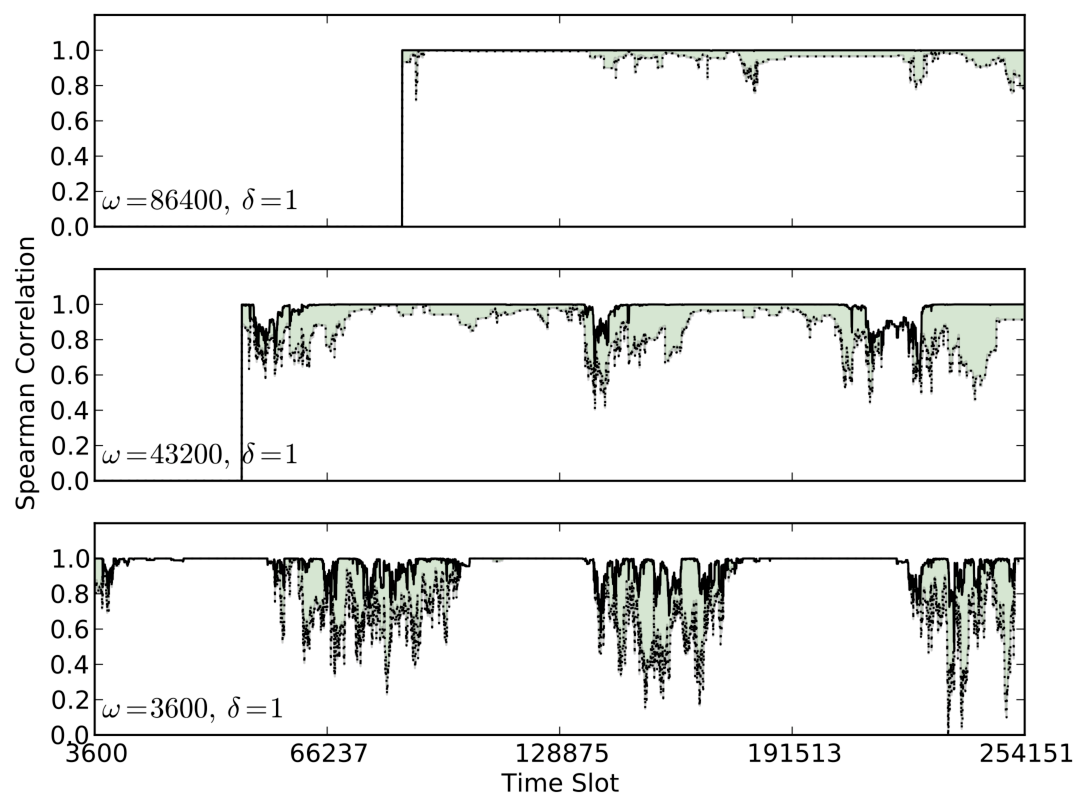
\includegraphics[width=0.49\linewidth, trim=0cm 0cm 0cm 0cm]{cor_spearman_time-step-1.pdf}}
\subfigure[{\em Step size $\delta=3600~seconds\,(=1~hour)$}]{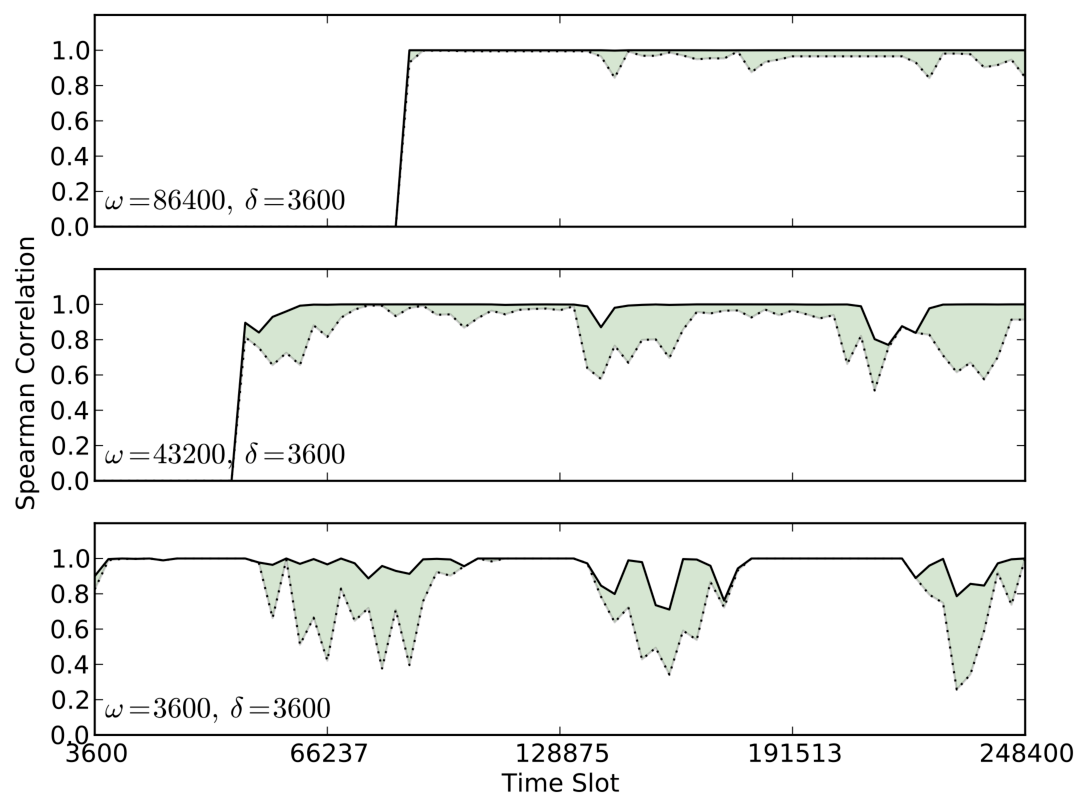
\includegraphics[width=0.49\linewidth, trim=0cm 0cm 0cm 0cm]{cor_spearman_time-step-3600.pdf}}
\caption{Change of correlation between different betweenness metrics over time (the solid line represents the correlation between x-ego betweenness and betweenness whereas the dotted line represents the correlation between ego betweenness and betweenness)}
\label{correlation_gap}
\end{figure*} 
Given a data set, our evaluations identified, for each time window $T_i$, social links between nodes.
In this case, any pair of nodes that communicated with each other for $\theta \cdot \omega / \pi$ time slots or more were assumed to have a social link between them.
On the network consisting of the above nodes and social links, our evaluations then computed the betweenness, ego-betweenness, and x-ego betweenness of each node using the Brandes algorithm~\cite{Brandes01afaster}.
The x-ego betweenness of each node was also computed using our algorithm (Section~\ref{computation}) to experimentally verify the benefit of that algorithm over the Brandes algorithm.

% ///////////////////////////////////
% 
% [older version]
% 
% For all data sets, we convert the original trace data into discrete sequential contact events per unit time per each node pair, and we feed them into each DTN node implemented in our simulation. 
% In a DTN node, the time is discretely slotted in unit of $1$ second from the start time $t_s (=0)$ until the end time $t_e (=\pi)$. For example, $\pi=254,151$ for the {\em Infocom05} data set. 
% %Each node maintains its own clock time, but shares the same length of time slot.\footnote{In real implement, time synchronization over all nodes is not required strictly, but a sophisticated synchronization scheme may help construct more precise ego or x-ego network.} 
% 
% Assuming that each contact lasts one time slot (i.e., each contact starts and ends during the same time slot), {\em a contact between two nodes $v$ and $k$ at time $t_o$} is defined as a 3-tuple $\langle v, k, t_o\rangle$ in our evaluations.\footnote{In spite of asymmetric communication characteristics in general, we assume that reception of a message guarantees a bidirectional contact for the sake of simplicity, like other studies \cite{human_mobility,SIMBET,IEEE:bubble} based on nodes' social behavior.} 
% DTN nodes aggregate its contacts during a {\em time window}, a set of contiguous time slots. 
% The time window size $\omega$ is constant in our simulation and empirically determined in real implement. 
% When time goes by, the time window slides by $\delta$ time slots (i.e., $\delta$ is also called as step size). 
% %If $\delta$ is small, a node will accurately construct its social networks according to its contact behavior, but high computational load will be imposed on each node. Since a node will configure its ego or x-ego network based on contact information in a time window, the social networks will become outdated if the value of $\delta$ is large, but each node can save its CPU cycles. 
% If $\delta$ is small, a node constructs its social networks accurately according to its contact behavior. On the other hand, social networks tend to be outdated if the value of $\delta$ is large.
% Let $T_{0}, T_{1}, \ldots$ denote the ordered sequence of time windows maintained by a node and the $i$th time window $T_{i}$ is defined as follows: $T_i=\{t_{\delta \cdot i}, t_{\delta \cdot i + 1}, t_{\delta \cdot i + 2}, \cdots, t_{\delta \cdot i + \omega - 1}\}$ where $0 \leq i \leq \lfloor\frac{\pi - \omega + 1}{\delta}\rfloor$.
% 
% For a time window $T_i$, a node $v$ maintains its contact duration time $d_{i,k}$ for each node $k$ which $v$ makes a contact during $T_i$. By the definition of contact, $d_{i,k}$ is the number of contacts $\langle v, k, t_o\rangle$ where $t_{\delta \cdot i} \leq t_o \leq t_{\delta \cdot i+\omega-1}$ and it is used to determine its {\em social neighbor nodes} for $T_i$. A node has a predefined threshold $\theta\cdot\omega/\pi$ and sorts out the social neighbor nodes $k'$ where $d_{i,k'} > \theta\cdot\omega/\pi$ at the every end of $T_i$. As explained previously, $\theta$ is pre-determined as a value given by Table \ref{data_set}. For a time window $T_i$, we will denote {\em a set of identifiers of social neighbor nodes} by $N_{v,i}$. 
% 
% %In SimBetTS \cite{SIMBET}, a well-known DTN forwarding scheme based on social graphs, a social link between two nodes is created if there has been at least any contact between them at any time in the past. That is, there is a single time window and $\omega$ is the whole duration of network operation (i.e., $\omega=\pi$). It means that SimBetTS does not consider the time window strategy and the constructed social graphs may get meshed since the whole network operation time contributes to the link creation. Another well-known social network based DTN routing, BUBBLE Rap \cite{IEEE:bubble}, used the similar time window as $T_i$ defined by this section. In the simulation of BUBBLE Rap, both of $\omega$ and $\delta$ were set to the number of time slots corresponding to $6~hours$. It means that two nodes may compare their centrality by using social metrics computed in relatively old time (i.e., $6~hours$ ago). In the two DTN routing schemes, the authors did not consider the quality of social graph fully. In this paper, we vary the values of $\omega$ and $\delta$ so that the diverse social graphs can be evaluated to prove the contribution of this paper. 
% 
% %In the whole simulation time, a DTN node sends {\em Hello} broadcast message periodically with interval of $\tau$ time slots. Each Hello message contains the following information: 1) {\em its own identifier} and 2) {\em a set of identifiers of social neighbor nodes}, the latter of which will be needed by a DTN node to construct its ego or x-ego network. In our simulation, we set $\tau$ to one.
% %During evaluation time, a DTN node sends {\em Hello} broadcast message including its own identifier periodically with interval of $\tau$ time slots. 
% %In our evaluation, we set $\tau$ to one.
% %Since an ego or x-ego network is constructed based on the information about such social neighbor nodes, a node should piggyback $N_{v,i}$ determined at the every end of $T_i$ into the broadcast messages sent during $T_{i+1}$. 
% For each node $k$ which $v$ makes a contact during $T_{i+1}$, $N_{k,i}$ determined at the end of $T_i$ is piggybacked into the contacts $\langle v, k, t_o'\rangle$ made during $T_{i+1}$ where $t_{\delta \cdot (i+1)} \leq t_o' \leq t_{\delta \cdot (i+1)+\omega-1}$ and it is used to configure $v$'s ego and x-ego networks during $T_{i+1}$.
% Since the social neighbor nodes are determined during the previous time window, information in $N_{v,i}$ will be more fresh if the step size $\delta$ of time window is small. At every end of time window $T_i$, $v$ also builds the array $N$ (an input parameter of Algorithm \ref{alg:main}) from $N_{v,i}$ and executes the proposed algorithm. The global network to be compared with ego or x-ego network is also constructed every end of time window $T_i$ by combining all the vertices and edges corresponding to $N_{v,i}$ created by all nodes.    
% 
% ///////////////////////////////////

\subsection{Accuracy of X-Ego Betweenness}\label{accuracy}
\begin{figure*}[t] 
\centering 
\subfigure[{\em Infocom05}]{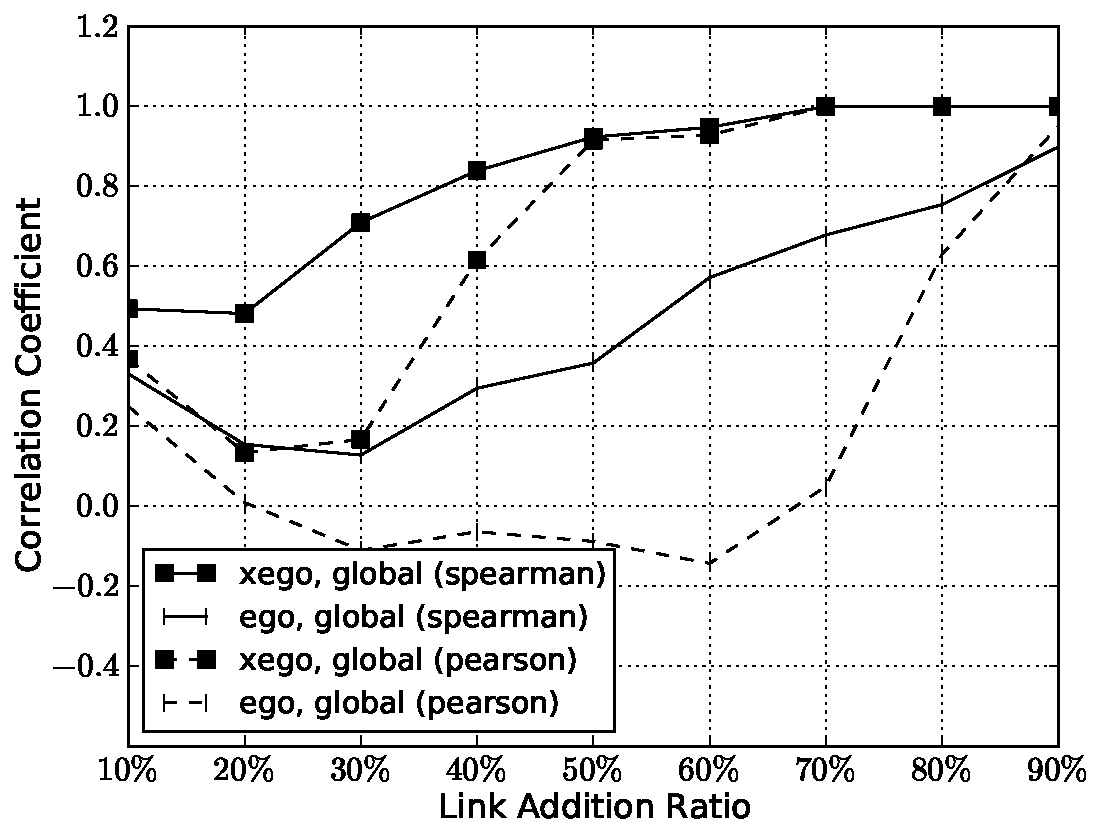
\includegraphics[width=0.246\linewidth, trim=0cm 0cm 0cm 0cm]{1_correlation.pdf}}
\subfigure[{\em Infocom06}]{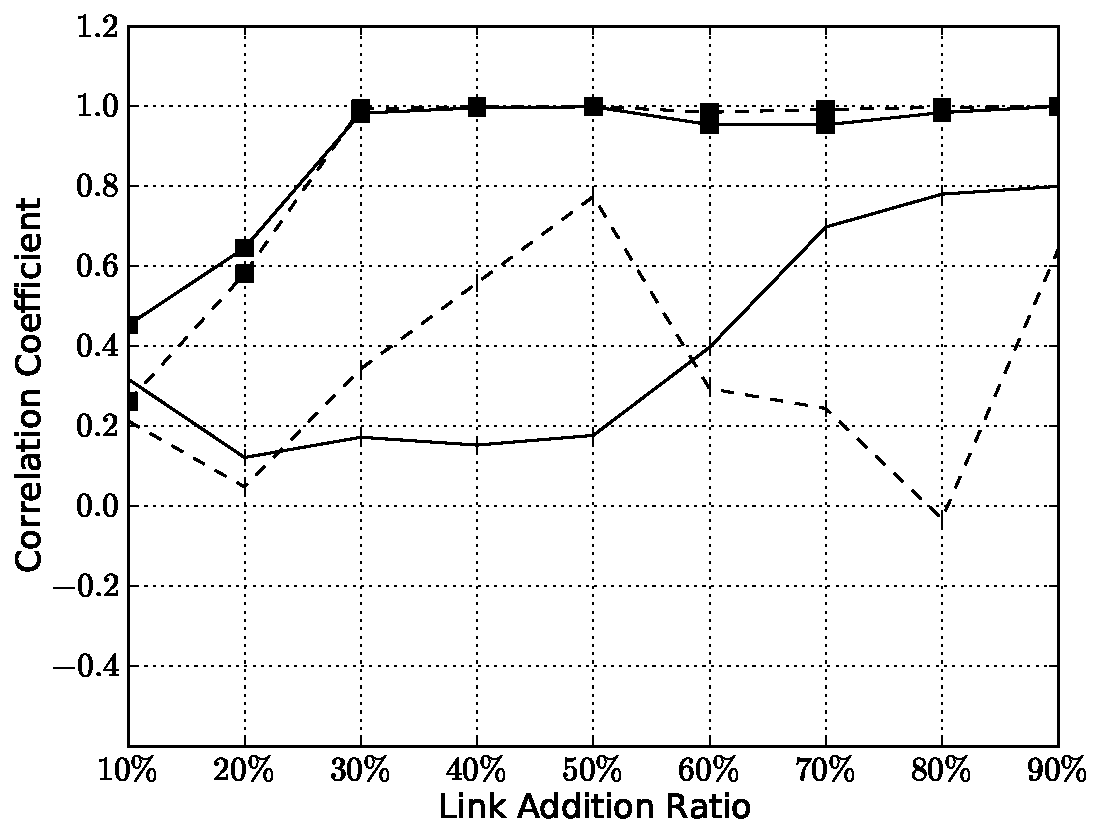
\includegraphics[width=0.246\linewidth, trim=0cm 0cm 0cm 0cm]{2_correlation.pdf}}
\subfigure[{\em Cambridge}]{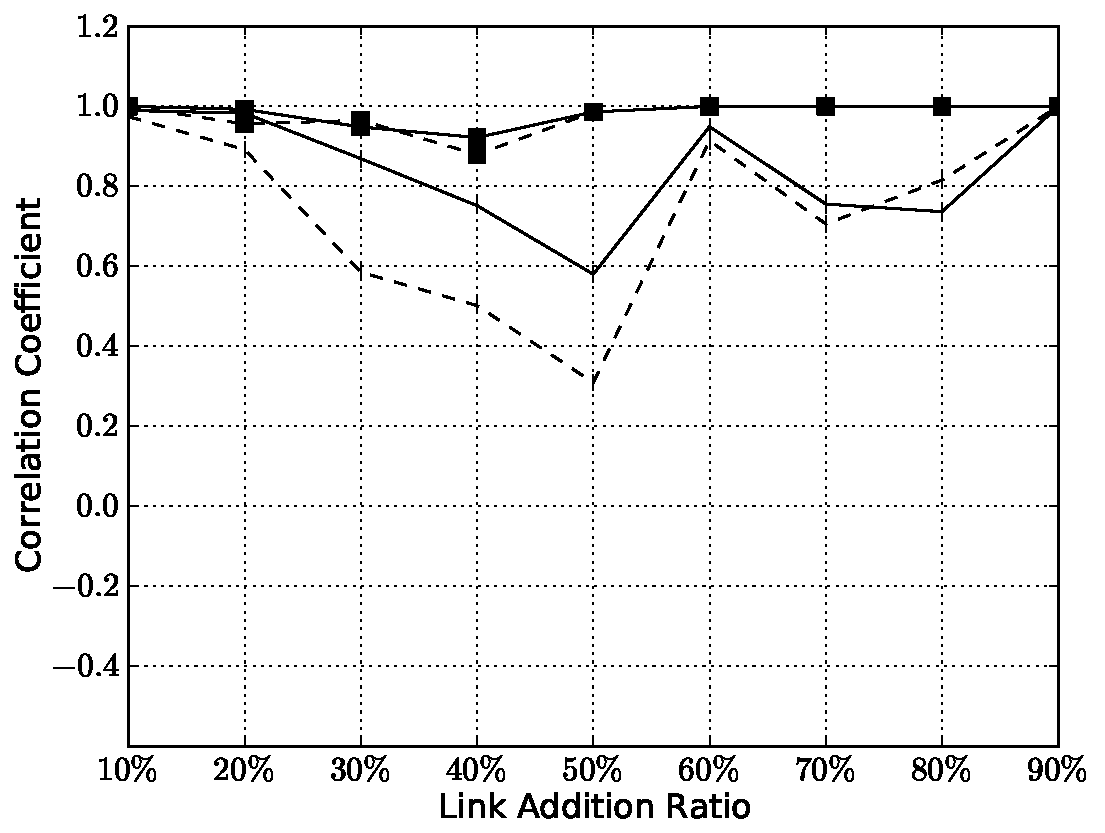
\includegraphics[width=0.246\linewidth, trim=0cm 0cm 0cm 0cm]{3_correlation.pdf}}
\subfigure[{\em Intel}]{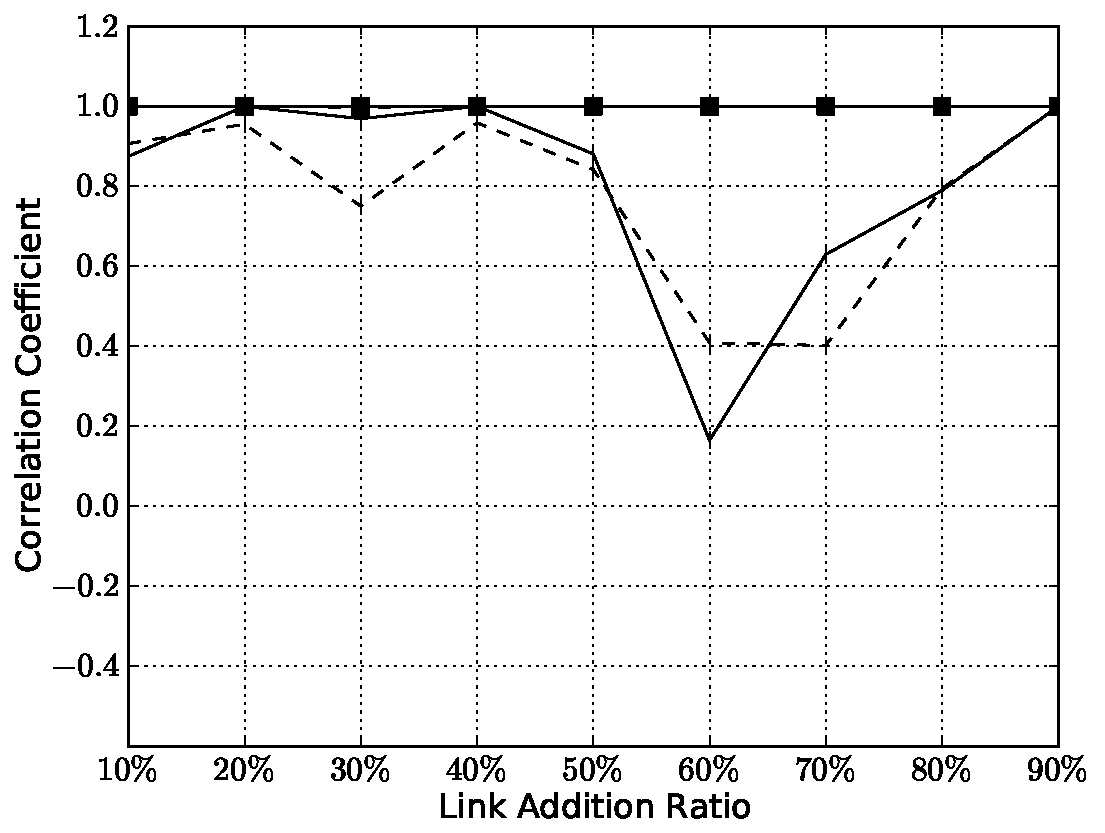
\includegraphics[width=0.246\linewidth, trim=0cm 0cm 0cm 0cm]{4_correlation.pdf}}
\caption{Correlation between different betweenness metrics ($\omega=\pi$)}
\label{correlation_comp}
\end{figure*} 

\begin{figure*}[t]
\centering 
\subfigure[{\em Infocom05}]{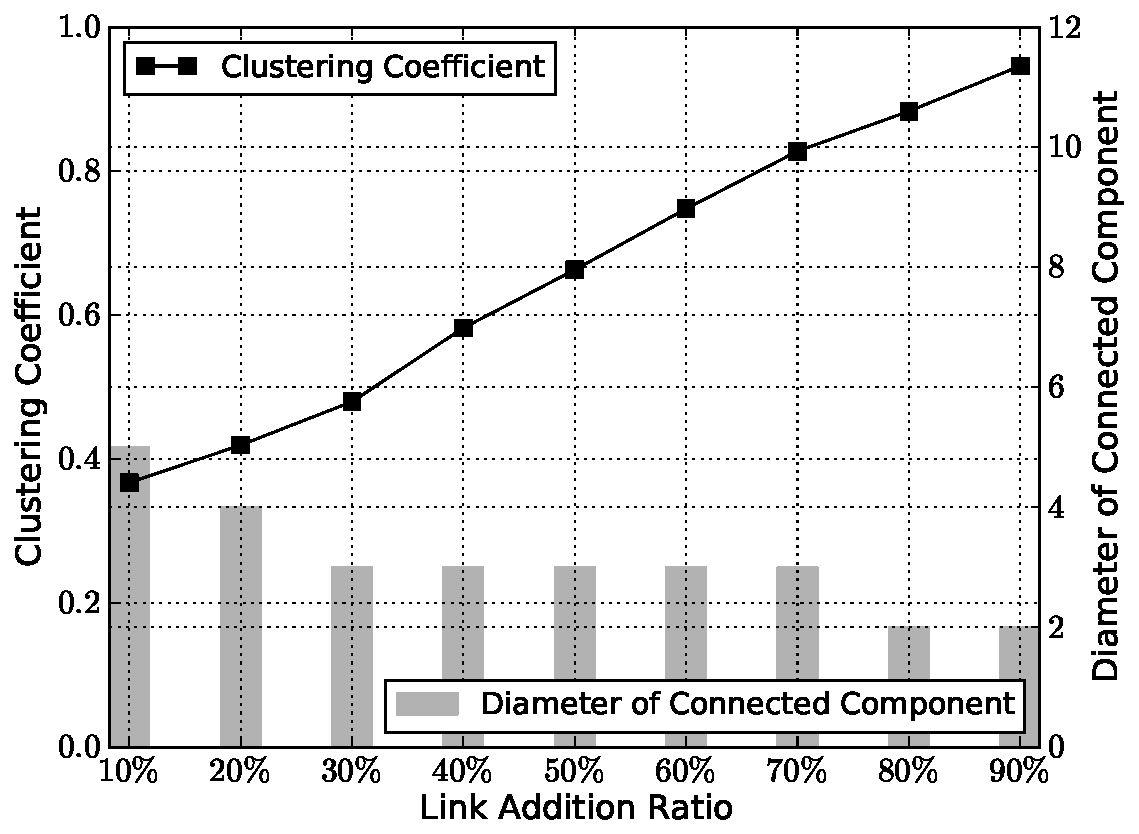
\includegraphics[width=0.246\linewidth, trim=0cm 0cm 0cm 0cm]{1_clustering_and_diameter.pdf}}
\subfigure[{\em Infocom06}]{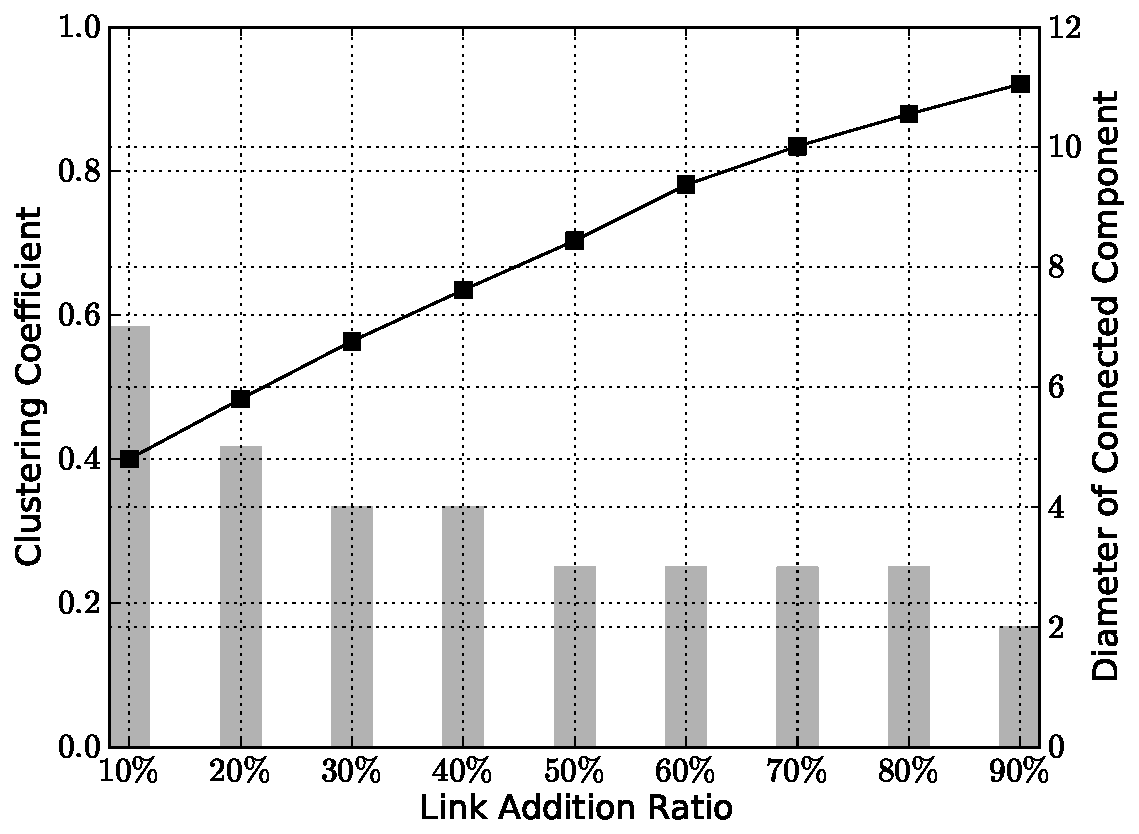
\includegraphics[width=0.246\linewidth, trim=0cm 0cm 0cm 0cm]{2_clustering_and_diameter.pdf}}
\subfigure[{\em Cambridge}]{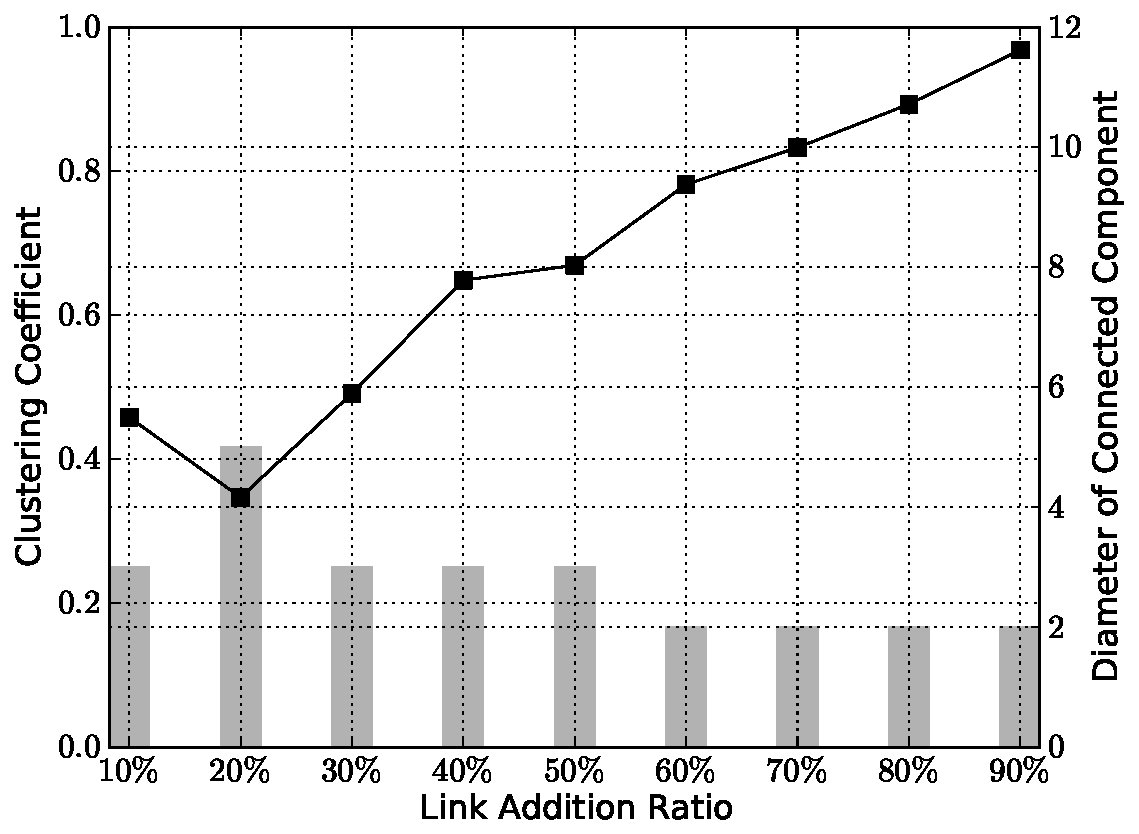
\includegraphics[width=0.246\linewidth, trim=0cm 0cm 0cm 0cm]{3_clustering_and_diameter.pdf}}
\subfigure[{\em Intel}]{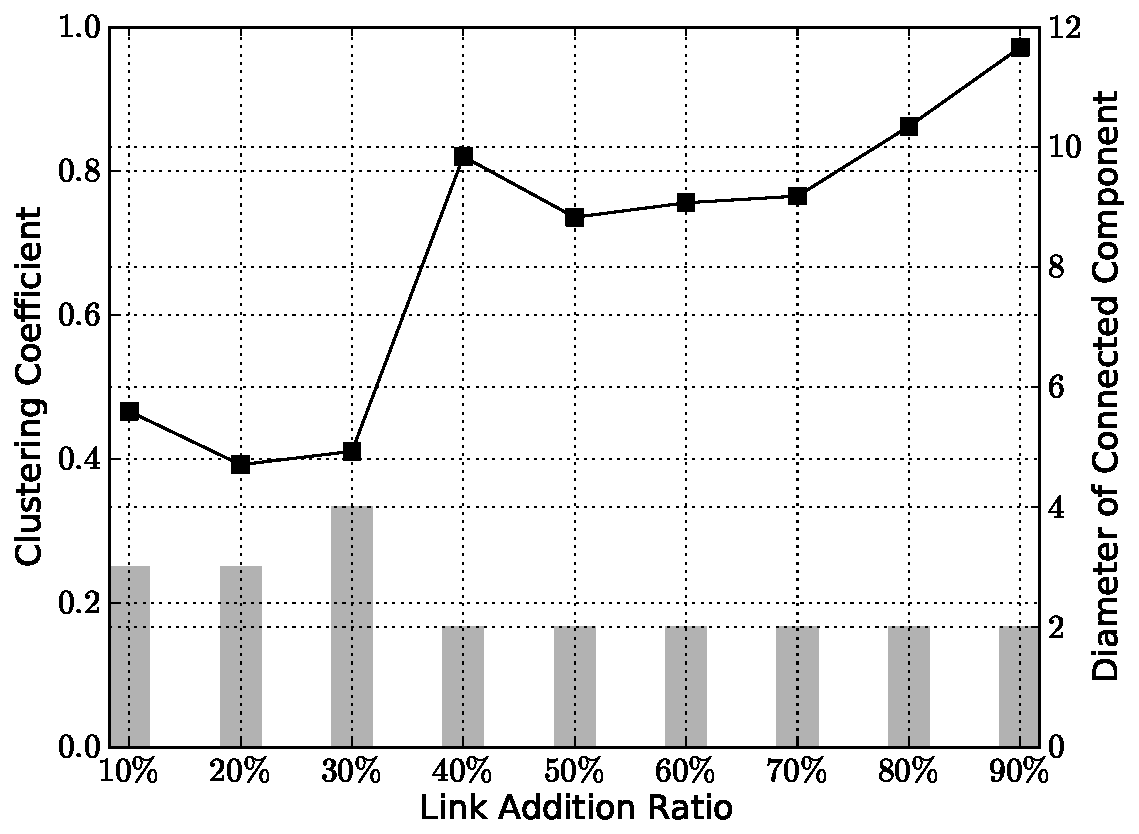
\includegraphics[width=0.246\linewidth, trim=0cm 0cm 0cm 0cm]{4_clustering_and_diameter.pdf}}
\caption{Clustering coefficient and diameter of  connected component ($\omega=\pi$)}
\label{netinfo1}
\end{figure*} 

\begin{figure*}[t] 
\centering 
\subfigure[{\em Infocom05}]{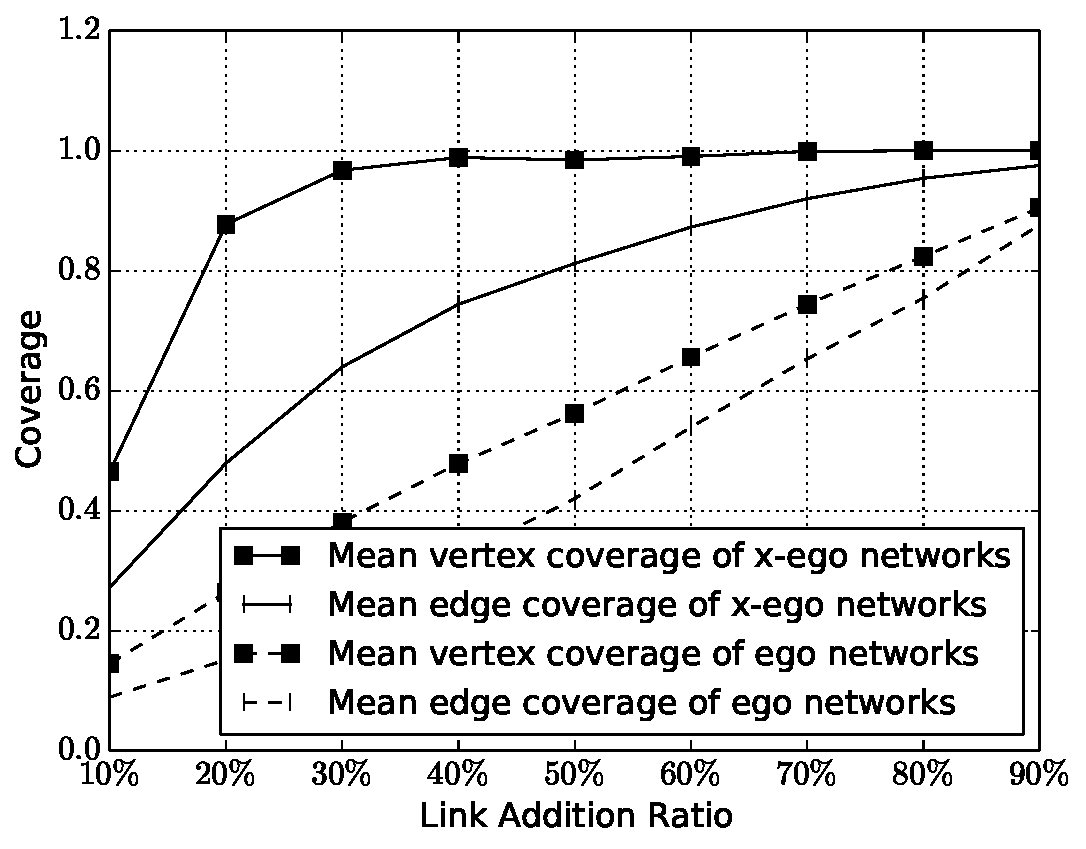
\includegraphics[width=0.246\linewidth, trim=0cm 0cm 0cm 0cm]{1_graph_info_2.pdf}}
\subfigure[{\em Infocom06}]{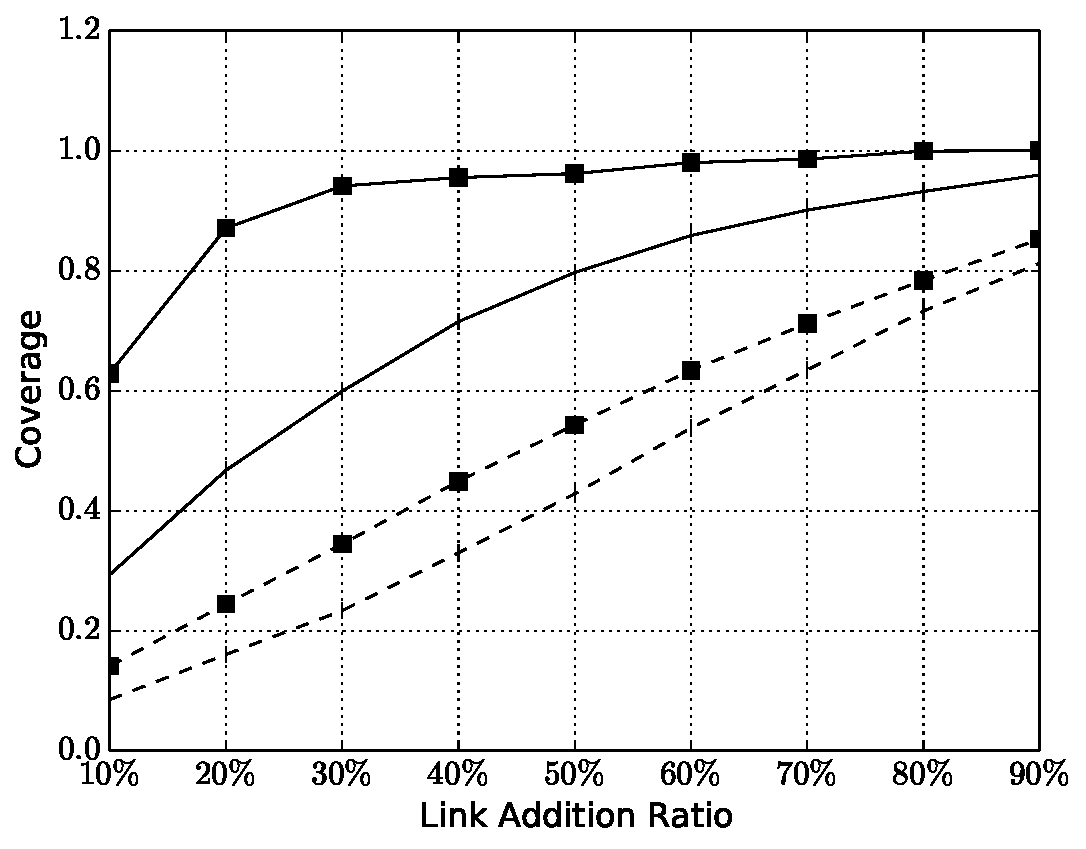
\includegraphics[width=0.246\linewidth, trim=0cm 0cm 0cm 0cm]{2_graph_info_2.pdf}}
\subfigure[{\em Cambridge}]{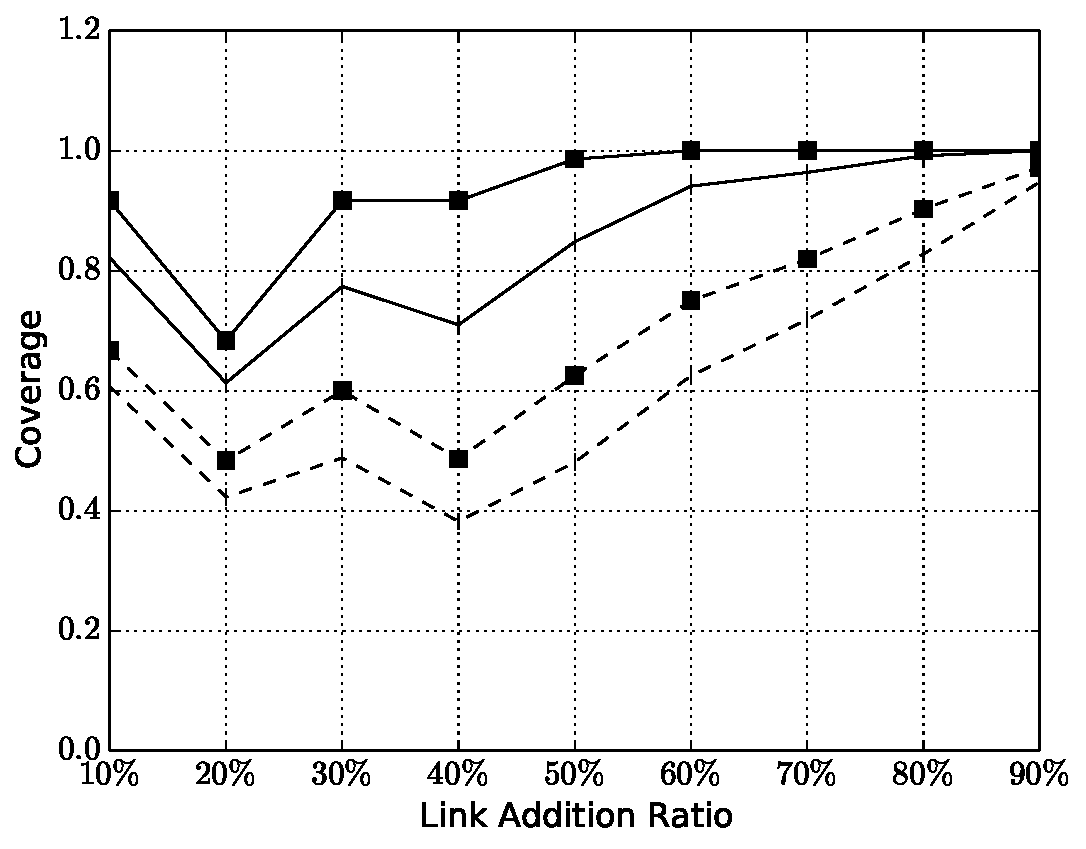
\includegraphics[width=0.246\linewidth, trim=0cm 0cm 0cm 0cm]{3_graph_info_2.pdf}}
\subfigure[{\em Intel}]{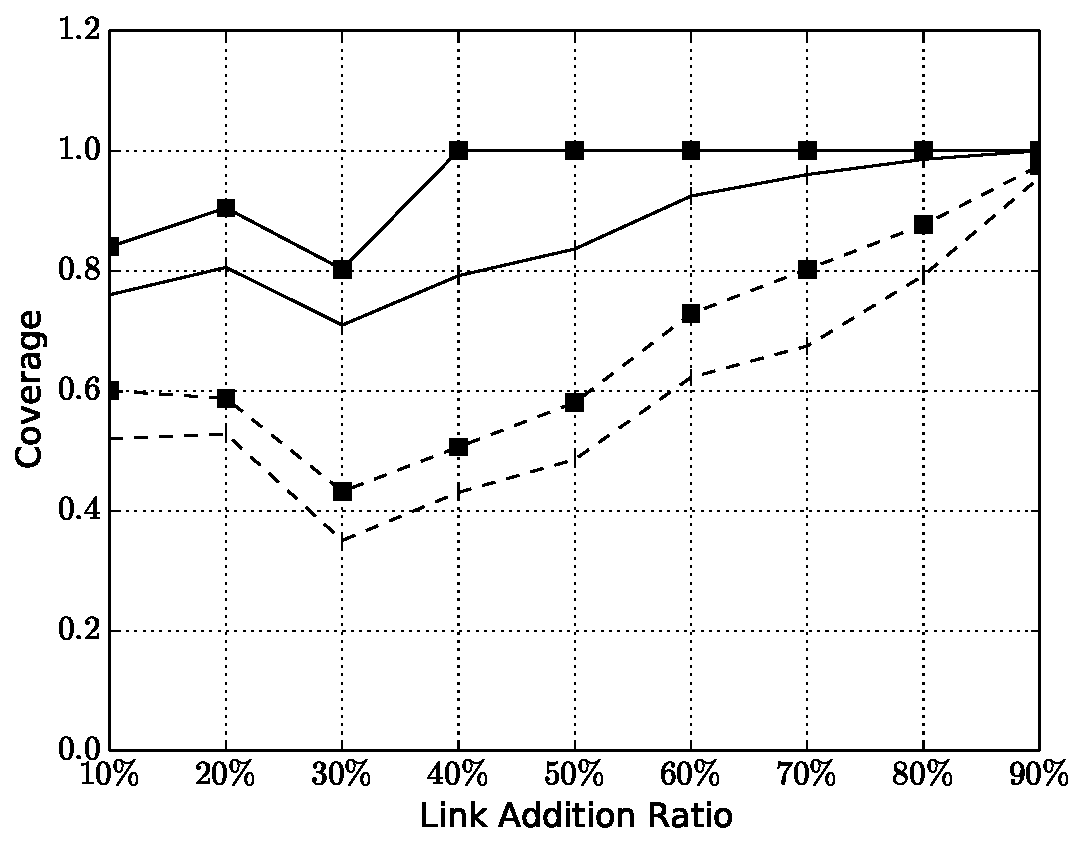
\includegraphics[width=0.246\linewidth, trim=0cm 0cm 0cm 0cm]{4_graph_info_2.pdf}}
\caption{Coverage of x-ego and ego networks over the global network ($\omega=\pi$)}    
\label{netinfo2}
\end{figure*}
%, $\NX$ and $\MX$: the average number of vertices and edges in x-ego networks, $\NE$ and $\ME$: the average number of vertices and edges in ego networks, $\NC$ and $\MC$: the average number of vertices and edges in connected components when, for each node, the connected component containing that node is considered
% Fig.~\ref{correlation_gap} shows the variation of gap between the Spearman correlation between $\BX{v}$ and $\B{v}$ and the one between $\BE{v}$ and $\B{v}$ over time slots. 
Fig.~\ref{correlation_gap} compares the accuracy of x-ego betweenness and ego betweenness in terms of their similarity to betweenness.
Each subfigure in Fig.~\ref{correlation_gap} shows the variation of the Spearman correlation between x-ego betweenness and betweenness (the dotted line) and that between ego betweenness and betweenness (the solid line).
% The data set {\em Infocom05} is used with time window size $\omega$ set to $86,400\,sec.\,(=24\,hours)$, $43,200\,sec.\,(=12\,hours)$ or $3,600\,sec.\,(=1\,hour)$, and step size $\delta$ set to $1\,sec.$ or $3,600\,sec$. 
The results illustrated in the figures were obtained from the {\em Infocom05} data set with the time window size $\omega$ set to 24 hours (86,400 seconds), 12 hours (43,200 seconds), or 1 hour (3,600 seconds) and the step size $\delta$ set to 1 second or 3,600 seconds.
% Edge creation ratio is $50\%$ so that a DTN node makes a social link with other node if the accumulated contact duration time is more than $1,609\cdot86,400/3,600\, (=38,616\,sec.)$ when $\omega=86,400$ and $\delta=3,600$. 
Furthermore, the link addition ratio was set to $50\%$ (equivalently, the contact duration threshold was set to 1,609 seconds).
For this reason, when $\omega=86{,}400$ and $\delta=3{,}600$, a node assumed a social link with another node if the accumulated contact duration between these nodes was longer than $1{,}609 \cdot 86{,}400 / 254{,}151\, (=546.9)$ seconds. 
% In each figure, there are two lines, each of which represents the spearman correlation between $\BX{v}$ and $\B{v}$, and between $\BE{v}$ and $\B{v}$, respectively. 
% We fill the space between the two lines to make the gap between them obvious. 

% It is observed in the figure that $\BX{v}$ is more correlated to $\B{v}$ than $\BE{v}$, which also means $\BX{v}$ is more accurate than $\BE{v}$.
Fig.~\ref{correlation_gap} shows that x-ego betweenness is more strongly correlated to betweenness than ego betweenness (i.e., x-ego betweenness is more accurate than ego betweenness) across different time window sizes and step sizes.
As the window step size ($\delta$) increases from 1 second (Fig.~\ref{correlation_gap} (a)) to 3,600 seconds (Fig.~\ref{correlation_gap} (b)), the betweenness of each vertex is computed/updated less frequently, thereby saving communication and computation resources at the expense of timeliness of betweenness values. 
% We can also know that both correlation values become very high when the time window size gets long. 
% It is because a DTN node can determine its local centrality more accurately if it uses sufficient information in a large window size. 
When the window step size ($\delta$) is fixed, as the time window size ($\omega$) increases, the variation of correlation between x-ego betweenness and betweenness decreases since the overlap between consecutive windows increases.
Given a larger time window, the correlation between x-ego betweenness and betweenness also increases since the x-ego network of each node may include more nodes (i.e., the accuracy of x-ego betweenness may improve).
% It also shows higher correlation values as the time window size ($\omega$) increases.
% In addition to that, the values are invariable since sliding step is not much high in comparison with the time window size and the past contact information is still used to get the values. 
%On the other hand, the correlation values become low and variable when the time window size gets short. 
% Even though the time window size is short, however, the correlation between $\BX{v}$ and $\B{v}$ is not much low: just $2.8\%$ of correlation values between $\BX{v}$ and $\B{v}$ over time slots is less than 0.8 when $\omega=3600$ and $\delta=1$, and $7.5\%$ when $\omega=3600$ and $\delta=3600$. 
On the other hand, even with small time windows, the overall correlation between x-go betweenness and betweenness remains high. 
For example, in Fig.~\ref{correlation_gap}, only $2.8\%$ of correlation values between x-ego betweenness and betweenness are smaller than 0.8 when $\omega=3{,}600$ and $\delta=1$, and only $7.5\%$ when $\omega=3{,}600$ and $\delta=3{,}600$. 

% Fig.~\ref{correlation_comp} shows the Spearman and Pearson correlation variation over diverse edge creation ratio and data sets. 
Fig.~\ref{correlation_comp} shows the correlation between x-ego betweenness and betweenness as well as between ego betweenness and betweenness across diverse link addition ratios and data sets.
% In this evaluation, all contact information over simulation duration are included into only one time window (i.e., $\omega = 2.9, 3.9, 5.3$ and $4.2$ days for each data set, respectively). 
This result was obtained by considering all contact information from each data set using a time window that corresponds to the data collection period (i.e., $\omega = 2.9, 3.9, 5.3$ and $4.2$ days for {\em Infocom05}, {\em Infocom06},  {\it Cambridge} and {\it Intel}, respectively).
% For the edge creation ratio/threshold values, we used the same values as the ones shown in Table \ref{data_set}. 
For each combination of data set and link addition ratio, we used the contact duration threshold shown in Table \ref{data_set}. 
% From the evaluation results, we found the followings: 
% \begin{itemize}
%   \item[1)] $\BX{v}$ is more highly correlated to globally computed betweenness $\B{v}$ than $\BE{v}$.
%   \item[2)] The correlation value between $\BX{v}$ and $\B{v}$ is very high (almost one) in most cases and it is even always one when small number of nodes constitute the DTN network like {\em Cambridge} or {\em Intel}.
% \end{itemize}

Fig.~\ref{correlation_comp} illustrates that:
\begin{itemize}
  \item[1)] X-ego betweenness is more strongly correlated to betweenness than ego betweenness (i.e., x-ego betweenness is more accurate than ego betweenness).
  \item[2)] The correlation between x-ego betweenness and betweenness is almost one in most cases. 
Furthermore, in the cases of {\em Cambridge} and {\em Intel}, where a small number of nodes constitute a network, the correlation between x-ego betweenness and betweenness is very close to one across all link addition ratios.
\end{itemize} 
% These features make $\BX{v}$ a proper measure for social-aware DTN routing schemes making use of betweenness centrality as the core metric of forwarding policy, since they are not trying to compare the absolute centrality values of each node but rather to determine which nodes are more central than others. 
% On the other hand, it is observed the Spearman and Pearson correlations between $\BE{v}$ and $\B{v}$ are very low in many cases. 
In contrast to the high correlation between x-ego betweenness and betweenness, the correlation between ego betweenness and betweenness is noticeably low in many cases.
% For example, it is mostly below 0.8 in the all data sets, and also mostly below 0.6 in {\em Infocom05} and {\em Infocom06} data sets, respectively. 
For example, it is mostly below 0.8 for all of the data sets and also mostly below 0.6 for {\em Infocom05} and {\em Infocom06}.
% These results show that the data delivery efficiency could be not high if social-aware DTN forwarding schemes would rely on $\BE{v}$.
The above results indicate the superiority of x-ego betweenness over ego betweenness in wireless networks.


% As shown in Fig. \ref{correlation_comp}, the correlation values become high if more edges are included into ego or x-ego networks (i.e.,  the network becomes dense), while they are mostly very low when the network is sparse. 
% For example, the lowest value of Spearman correlation between $\BX{v}$ and $\B{v}$ is $0.4819$ and $0.4535$ when the edge creation ratio is $20\%$ at the {\em Infocom05} data set and $10\%$ at the {\em Infocom06} data set, respectively. 
% The lowest value in {\em Cambridge} data set are found even when the ratio is relatively high, i.e., $0.4$. 
% In order to understand these results better, we investigate diverse metrics on network structure,  and study the relation between the correlation and them. 
% The results are depicted in Fig. \ref{netinfo1} and \ref{netinfo2}. 
\begin{figure*}[t]
\centering
\subfigure[{\em Infocom05}]{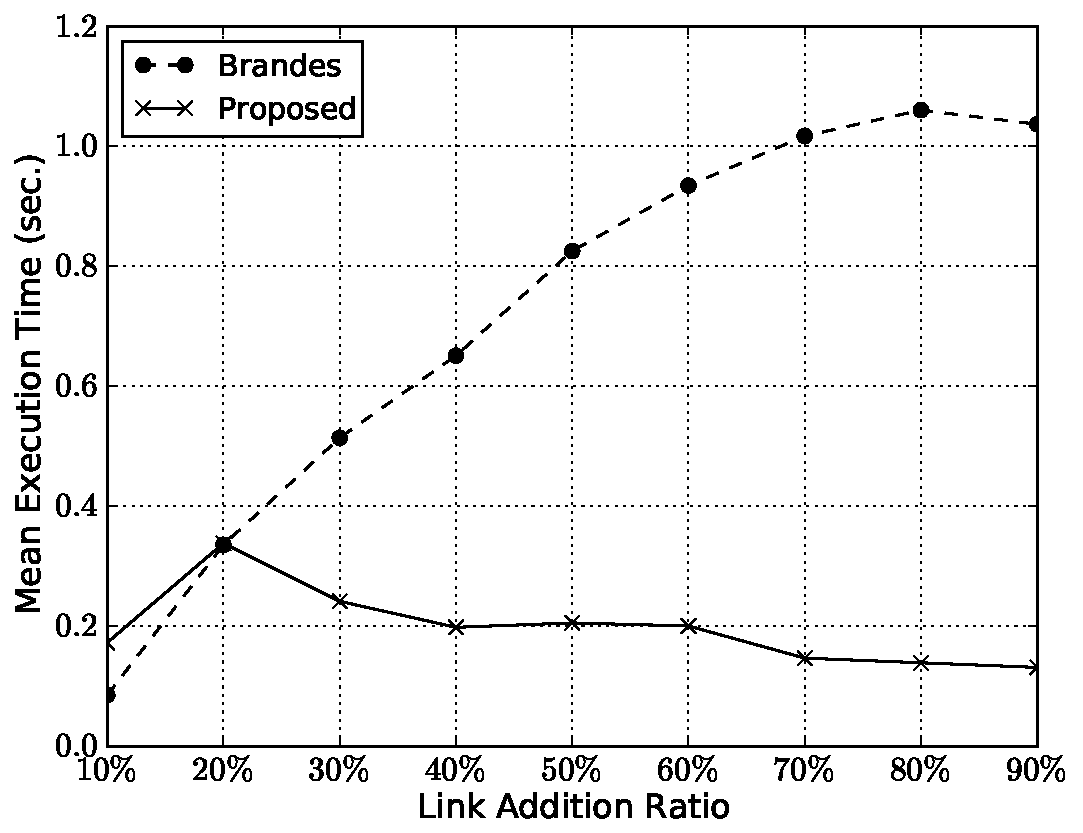
\includegraphics[width=0.24\linewidth, trim=0cm 0cm 0cm 0cm]{1_xEgo_elapsed_time.pdf}}
\subfigure[{\em Infocom06}]{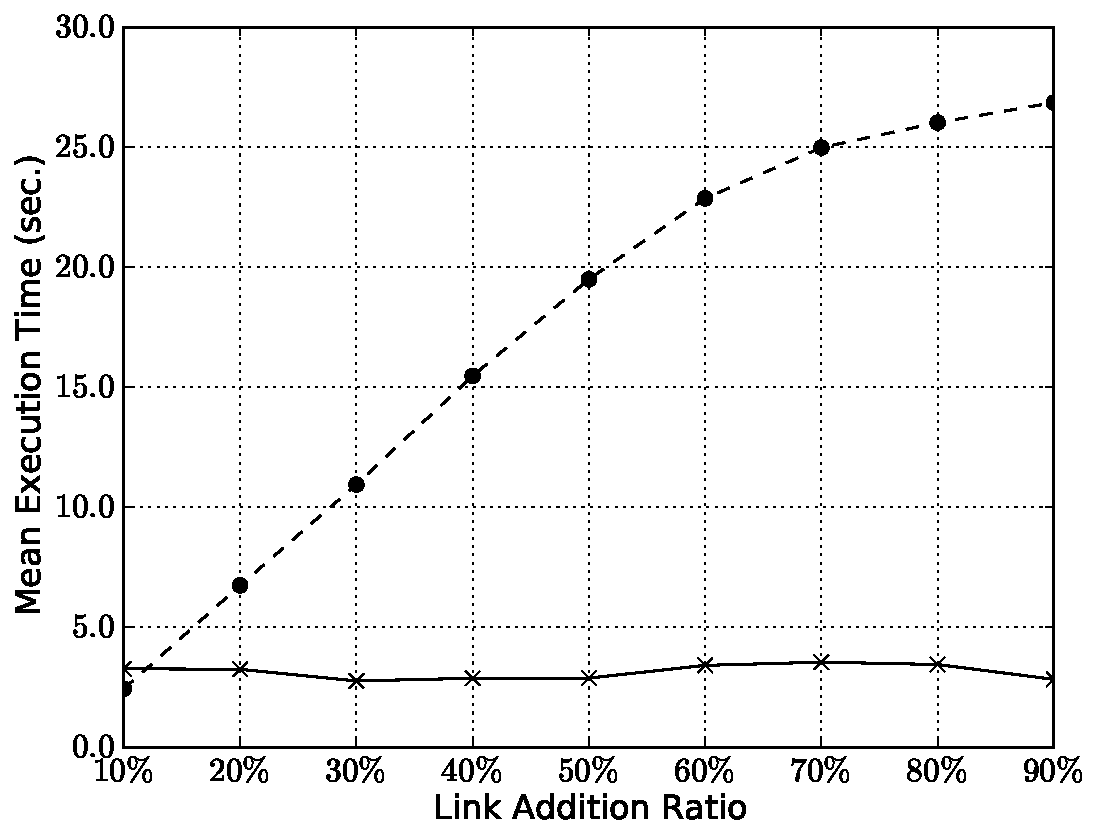
\includegraphics[width=0.243\linewidth, trim=0cm 0cm 0cm 0cm]{2_xEgo_elapsed_time.pdf}}
\subfigure[{\em Cambridge}]{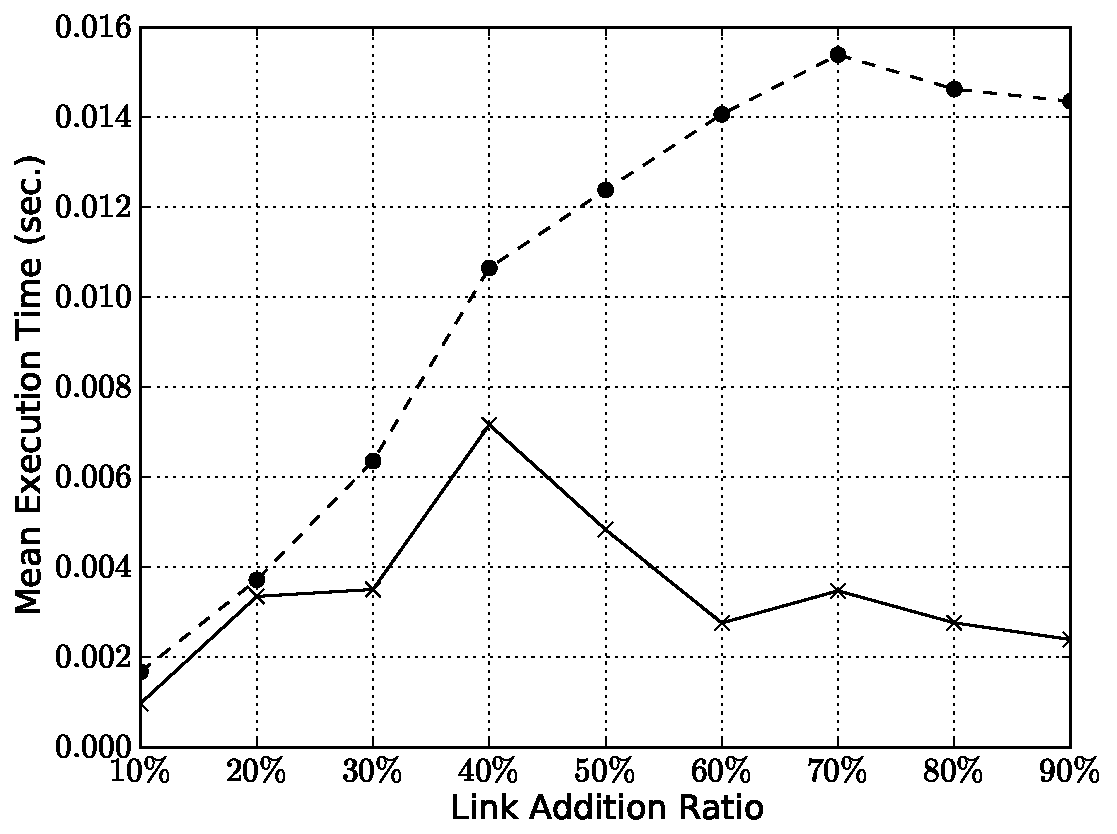
\includegraphics[width=0.247\linewidth, trim=0cm 0cm 0cm 0cm]{3_xEgo_elapsed_time.pdf}}
\subfigure[{\em Intel}]{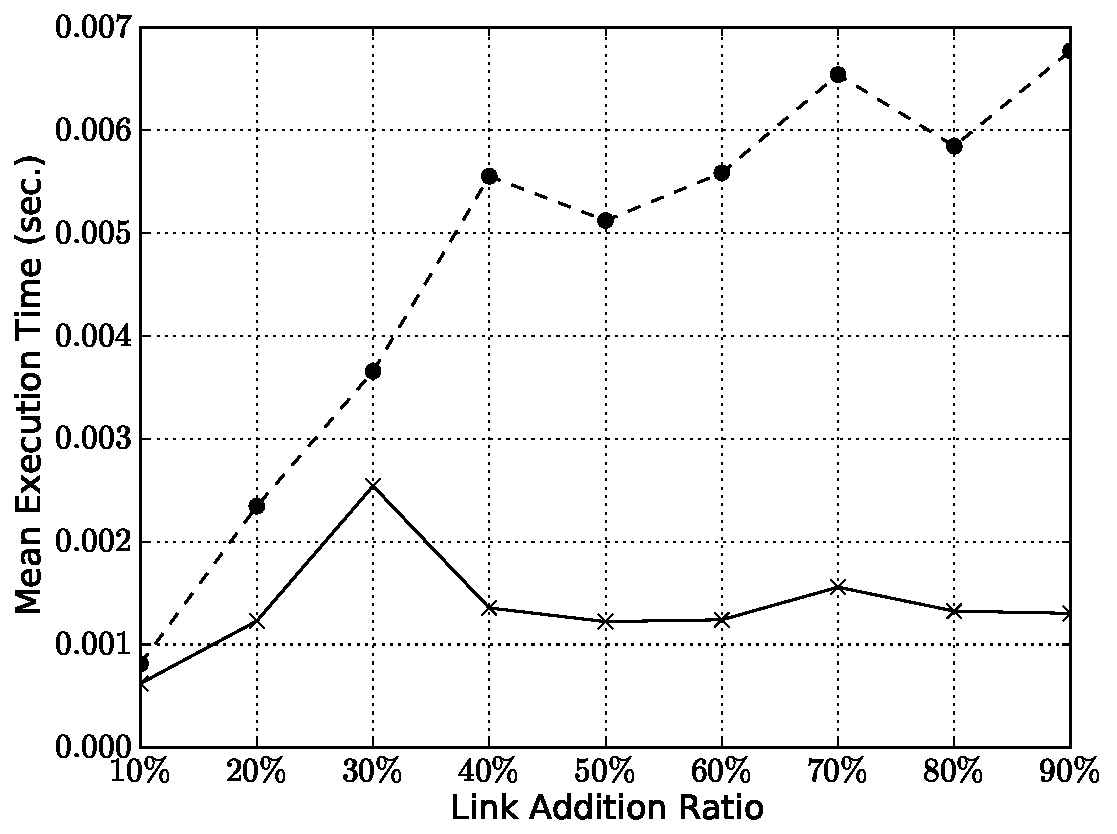
\includegraphics[width=0.247\linewidth, trim=0cm 0cm 0cm 0cm]{4_xEgo_elapsed_time.pdf}}
\caption{Comparison of algorithm execution speed to get x-ego betweenness}
\label{speed}  
\end{figure*}

\begin{figure*}[t]
\centering
\subfigure[{\em Infocom05}]{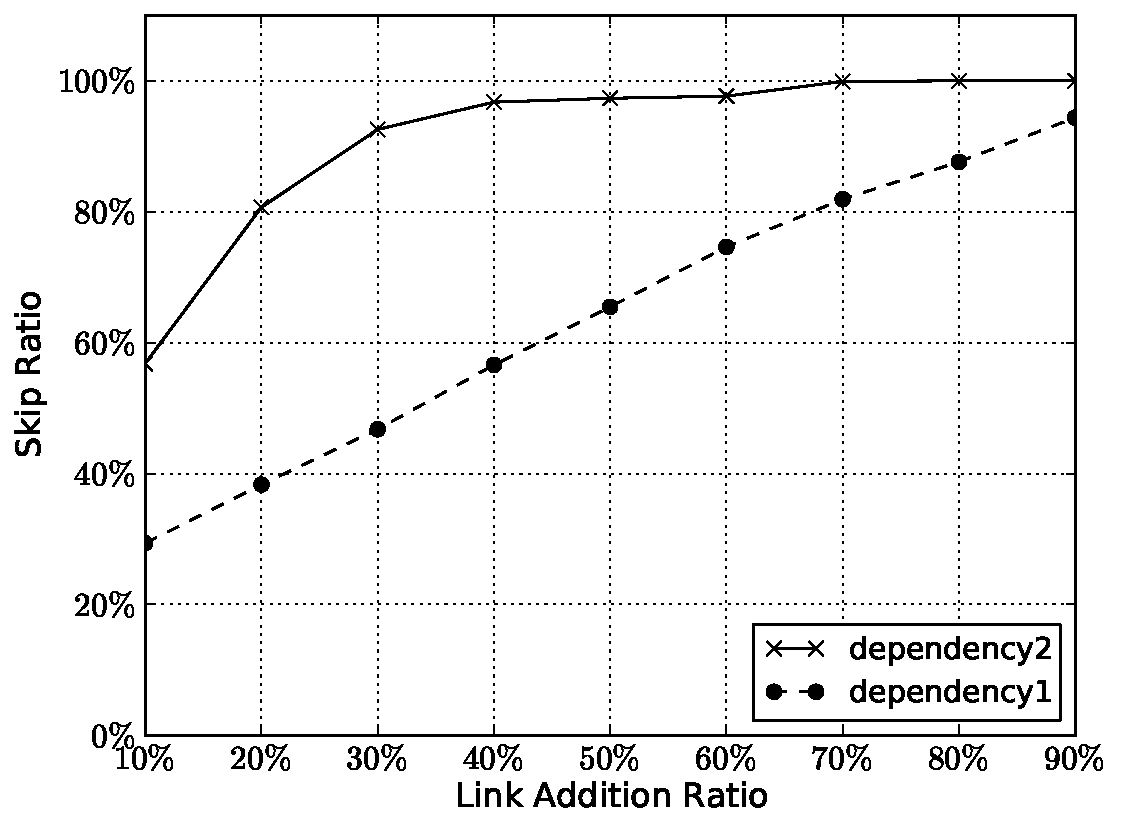
\includegraphics[width=0.246\linewidth, trim=0cm 0cm 0cm 0cm]{1_xEgo_skip_rate.pdf}}
\subfigure[{\em Infocom06}]{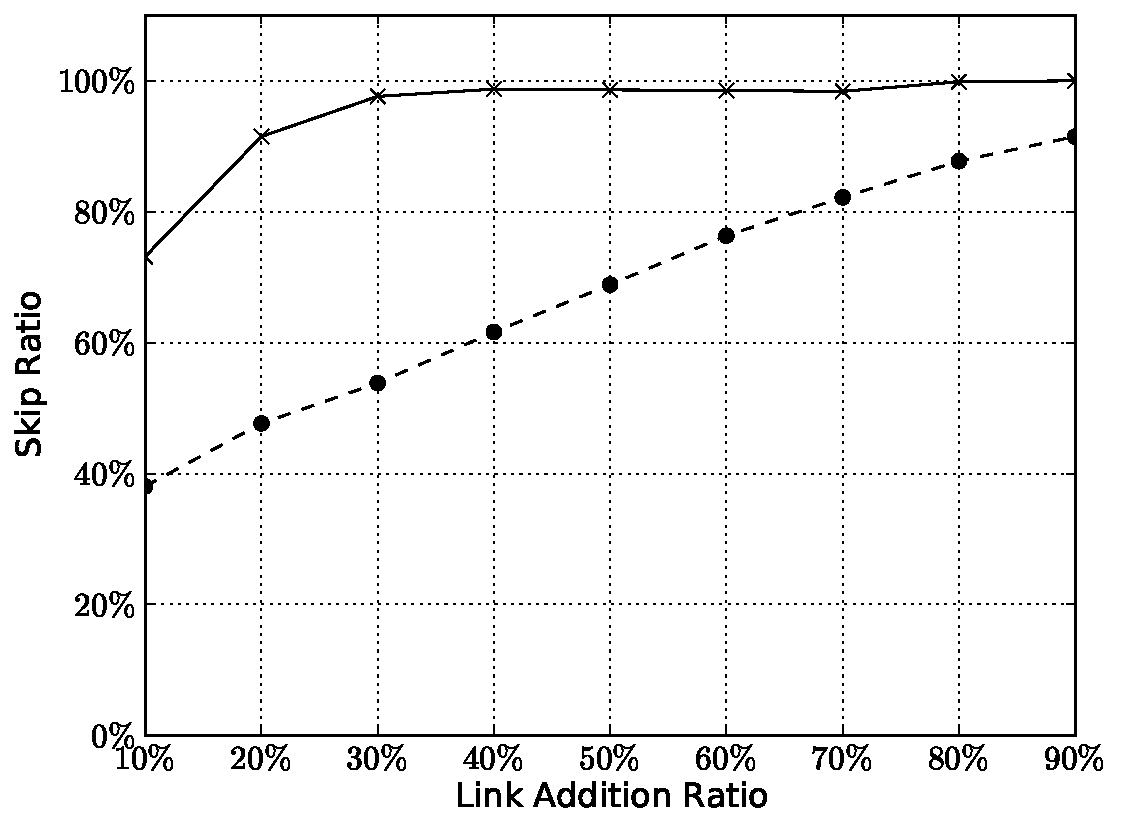
\includegraphics[width=0.246\linewidth, trim=0cm 0cm 0cm 0cm]{2_xEgo_skip_rate.pdf}}
\subfigure[{\em Cambridge}]{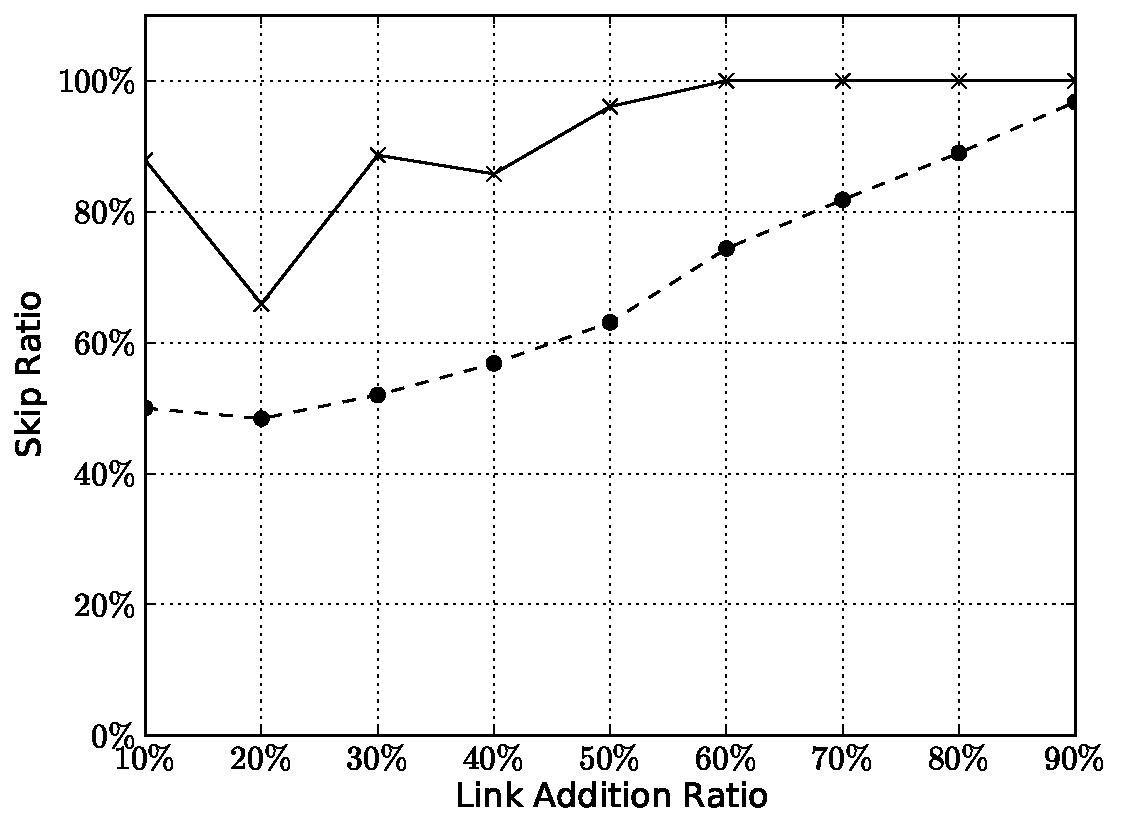
\includegraphics[width=0.246\linewidth, trim=0cm 0cm 0cm 0cm]{3_xEgo_skip_rate.pdf}}
\subfigure[{\em Intel}]{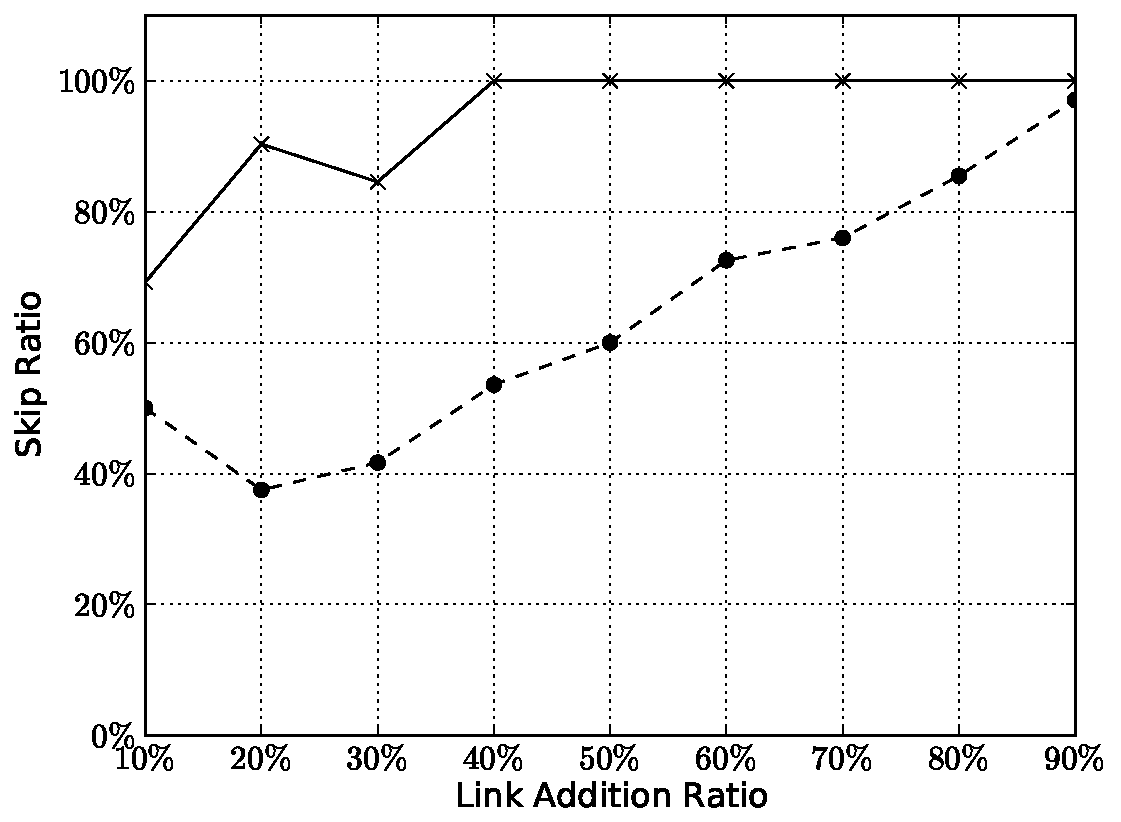
\includegraphics[width=0.246\linewidth, trim=0cm 0cm 0cm 0cm]{4_xEgo_skip_rate.pdf}}
\caption{Skip ratio in the proposed algorithm}
\label{skip}
\end{figure*}
 
In Fig.~\ref{correlation_comp}, while the same network overhead is required for both x-ego betweenness and ego betweenness (Section~\ref{x-ego_definition}), the correlation between x-ego betweenness and betweenness is consistently higher than the correlation between ego betweenness and betweenness. 
There are, however, link addition ratios (e.g., 10\% and 20\% in Fig.~\ref{correlation_comp} (a) and Fig.~\ref{correlation_comp} (b)) that lead to relatively low correlation between x-ego betweenness and betweenness.
To understand these situations, we obtained further evaluation results that are depicted in Fig.~\ref{netinfo1} and Fig.~\ref{netinfo2}. 

% Fig. \ref{netinfo1} shows the clustering coefficient and the diameter of the component in the global networks. When we compare a figure in Figure \ref{netinfo1} with the corresponding figure in Figure \ref{correlation_comp}, we can observe the followings:
% \begin{itemize}
% \item[1)] The correlation values are mostly proportional to the clustering coefficient of global network.
% \item[2)] The correlation values are mostly in inverse proportion to the network diameter of global network.
% \item[3)] The accuracy of $\BX{v}$ tends to be low when the network diameter of global network is more than 4.
% \end{itemize} Among the above findings, the third one is because x-ego networks include only 1 and 2-hop neighbors of a DTN node. Therefore, a DTN nodes need to keep the edge creation ratio more than roughly $30\%$. On the other hand, the above features are not distinct when the scale of network is low. 

Fig.~\ref{netinfo1} shows, for each data set, the impact of link addition ratio on the clustering coefficient and the average diameter of the connected components in the corresponding network.
As more links are added, the 1-hop neighbors of each node tend to have more links between them (i.e., the clustering coefficient increases) and the shortest path length between nodes tends to decrease (i.e., the diameter of the connected component containing the node decreases).\footnote{For the link addition ratio of 10\% in Figure~\ref{netinfo1} (c) and the same of 10\% and 20\% in Figure~\ref{netinfo1} (d), the network diameter is unusually small since, due to a very small number of links in the underlying network, each node has only a few reachable nodes and the latter are within 2 hops away from the former.}
Fig.~\ref{correlation_comp} and Fig.~\ref{netinfo1} show that x-ego betweenness and betweenness are strongly correlated when the average diameter of the connected components is less than 4.
In such cases, there is a large overlap between the x-ego network of a node and the connected component containing that node (i.e., x-betweenness is an accurate estimation of betweenness).
% As shown in Figure \ref{netinfo2}, we also examined two coverage ratios of ego or x-ego network to global network: 1) vertex coverage ($\NX/\NC$ and $\NE/\NC$) and 2) edge coverage ($\MX/\MC$ and $\ME/\MC$). 
% We can observe that x-ego networks cover most vertices in connected components containing the corresponding ego node in the global network, when the edge creation ratio is not low. 
% On the other hand, ego networks do not cover much vertices and edges in the connected components for most cases. 
% These coverage gaps become the fundamental reason that $\BX{v}$ is more highly correlated to globally computed betweenness $\B{v}$ than $\BE{v}$.

%Fig.~\ref{netinfo2} shows the size of x-ego and ego networks compared to the underlying DTN.
Fig.~\ref{netinfo2} shows the size of x-ego and ego networks compared to the global network. 
For this result, we found, for each node $v$, the number of vertices in the x-ego network of $v$ (denoted as $|\XN{v}(V)|$) and that in the ego network of $v$ (denoted as $|\EN{v}(V)|$) as well as the number of edges in the x-ego network of $v$ (denoted as $|\XN{v}(E)|$) and that in the ego network of $v$ (denoted as $|\EN{v}(E)|$).
We also obtained, for each node $v$, the number of vertices and that of edges in the connected component containing $v$ (denoted as $|\CC{v}(V)|$ and $|\CC{v}(E)|$, respectively) in the global network.
Then, the ``mean vertex coverage of x-ego networks'' and ``mean edge coverage of x-ego networks'' were computed as $\frac{\sum_{v \in V} \frac{|\XN{v}(V)|}{|\CC{v}(V)|}}{|V|}$ and $\frac{\sum_{v \in V} \frac{|\XN{v}(E)|}{|\CC{v}(E)|}}{|V|}$, respectively.
Furthermore, the ``mean vertex coverage of ego networks'' and ``mean edge coverage of ego networks'' were computed as $\frac{\sum_{v \in V} \frac{|\EN{v}(V)|}{|\CC{v}(V)|}}{|V|}$ and $\frac{\sum_{v \in V} \frac{|\EN{v}(E)|}{|\CC{v}(E)|}}{|V|}$, respectively.
Fig.~\ref{netinfo2} shows that, while ego and x-ego networks require the same network overhead (Section~\ref{x-ego_definition}), x-ego networks contain a substantially larger number of vertices and edges than ego networks (i.e., x-ego betweenness is a more accurate estimation of betweenness than ego betweenness).

\subsection{Efficiency of Our X-Ego Betweenness Algorithm}\label{efficiency}
% As known by the previous evaluation, the accuracy of $\BX{v}$ will be high if the scale of x-ego network is large. 
% However, its computation time becomes high accordingly. 
% So, we proposed a new algorithm to alleviate such computation time on x-ego networks in Section \ref{computation}. 
% In this section, we analyze the performance of the proposed algorithm.  
This section evaluates the performance benefit of our x-ego betweenness algorithm (Section~\ref{computation}).
To the best of our knowledge, no other x-ego betweenness algorithms have been proposed in the literature.
For this reason, we compare the performance of our algorithm to that of the Brandes algorithm~\cite{Brandes01afaster}, the state-of-the-art method for computing betweenness, while applying the latter to the x-ego network of each node. 
% Figure \ref{speed} depicts the average elapsed time for a DTN node $v$ to execute the Brandes algorithm and the proposed one to get its $\BX{v}$ on its x-ego network. 
Fig.~\ref{speed} shows the mean execution time of these algorithms (averaged over all nodes).
% For this evaluation, all contact information over simulation duration are also included into only one time window (i.e., $\omega=\pi$). 
For each data set, this evaluation result was obtained by using a time window that corresponded to the data collection period (i.e., $\omega=\pi$). 
% Like Fig. \ref{correlation_comp}, we plotted the elapsed times while changing the network density by adjusting the edge creation ratio from $10\%$ (sparse) to $90\%$ (dense).
As in Fig.~\ref{correlation_comp}, the link addition ratio was varied from $10\%$ (sparse) to $90\%$ (dense).
% As shown in the figure, the proposed algorithm has much lower elapsed time than the Brandes algorithm. 
% It is worth noting that the efficiency of the proposed algorithm is more conspicuous when x-ego networks become dense. 
% Sometimes, the elapsed time decreases even though x-ego networks become dense. 
Fig.~\ref{speed} shows that our algorithm is substantially faster than the Brandes algorithm.
In the figure, the benefit of our algorithm over the Brandes algorithm is more evident in dense networks (i.e., when the link addition ratio is high).
As the link addition ratio increases (i.e., the network density increases), the execution time of the Brandes algorithm increases.
On the other hand, the execution time of our algorithm may decrease in such cases.

% A DTN node needs to compute a set intersection in line 5 of Algorithm 2 (function {\em dependency1}) and compute a harmonic mean in line 15 of Algorithm 3 (function {\em dependency2}), which are {\em critical sections} of the proposed algorithm and make the overall elapsed time long. 
% However, such critical sections can be skipped when the conditions of Theorem 1 or 3 are satisfied. 
% We define {\em skip rate} as follows:
% \begin{equation}
% 1.0 - \frac{NUM_X}{NUM_C}.
% \end{equation} where $NUM_C$ is the number of function calls to {\em dependency1} or {\em dependency2}, and $NUM_X$ is the number of entries to the critical section of each function. 
To understand the above benefits of our algorithm, we further analyzed our evaluation results with a focus on $\frac{NUM_X}{NUM_C}$, which we call the {\em skip ratio}.
When {\em dependency1} (Algorithm~\ref{alg:dependency1}) is considered, $NUM_C$ denotes the number of dependency computations to which Theorems~\ref{theorem1} or \ref{theorem2} are applied and $NUM_X$ denotes the number of dependency computations to which only Theorem~\ref{theorem1} is applied (both $NUM_C$ and $NUM_X$ are determined while the x-ego betweenness of every node is calculated).
When {\em dependency2} (Algorithm~\ref{alg:dependency2}) is considered, $NUM_C$ denotes the number of dependency computations to which Theorems~\ref{theorem3} or \ref{theorem4} are applied and $NUM_X$ denotes the number of dependency computations to which only Theorem~\ref{theorem3} is applied.
As $NUM_X$ increases (i.e., Theorem~\ref{theorem1} or Theorem~\ref{theorem3} are more frequently applied), more expensive set operations (line 5 of Algorithm 2) and harmonic mean computations (line 15 of Algorithm 3) are skipped, thereby reducing the overall x-ego betweenness computation time.
 
% Fig. \ref{skip} plots the skip rate for the two function calls. 
% As shown in the figure, the skip rate of {\em dependency1} is mostly more than $80\%$ over the whole edge creation ratio and almost $100\%$ when the edge creation ratio is more than $50\%$. 
Fig.~\ref{skip} shows that the skip ratio for {\em dependency1} is in general higher than $80\%$ across all link addition ratios and is almost $100\%$ (i.e., the set intersection operation on line 5 of Algorithm 2 is very rarely performed) when the link addition ratio is higher than $50\%$. 
% If x-ego networks become dense, the possibility that two 1-hop neighbors of a node share en edge is high and the skip rate becomes high, too (see Theorem 1). 
In a dense x-ego network, the probability that two arbitrary 1-hop neighbors of a node share an edge is high (i.e., the skip ratio is high since Theorem~\ref{theorem1} applies frequently).
% Moreover, we can know that Algorithm 2 hardly contributes the elapsed time if the edge creation ratio is more than $50\%$. 
% Such high density of x-ego networks increases the likelihood to satisfy the condition of Theorem 3 high and hence enhance the skip rate of {\em dependency2}. 
In this case, the skip ratio for {\em dependency2} is also high as Theorem~\ref{theorem3} applies frequently.
% If the edge creation ratio is more than $50\%$, the skip rate of {\em dependency2} is more than $60\%$. 
In Fig.~\ref{skip}, the skip ratio for {\em dependency2} is higher than $60\%$ when the link addition ratio is higher than $50\%$. 
These high skip ratios account for the performance benefit of our x-ego betweenness algorithm in dense networks.
% From these results, we can know that the proposed algorithm is highly efficient when we get x-ego betweenness over x-ego networks.


% except the case of the Infocom05 dataset with the link generation threshold of $1/cd_{max}$. In the network configured with the dataset and the threshold, there are many nodes of which has many triads. Such triads can generate many shortest paths between nodes in the triads. This may make the ego or expanded ego betweenness low compared to the globally computed betweenness. 

%It is unusual but sometimes nodes make many triads with neighbors and these triads generate many geodesics. This phenomenon causes lowered ego or expanded ego betweenness value.
